%\thispagestyle{myheadings}
\section{Keynote Address: Ehud Reitter}
\index{Reitter, Ehud}

\begin{center}
\begin{Large}
{\bfseries\Large Evaluating Natural Language Generation Systems}
\vspace{1em}\par
\end{Large}

\daydateyear, 9:00--10:15am \vspace{1em}\\
\PlenaryLoc \\
\vspace{1em}\par
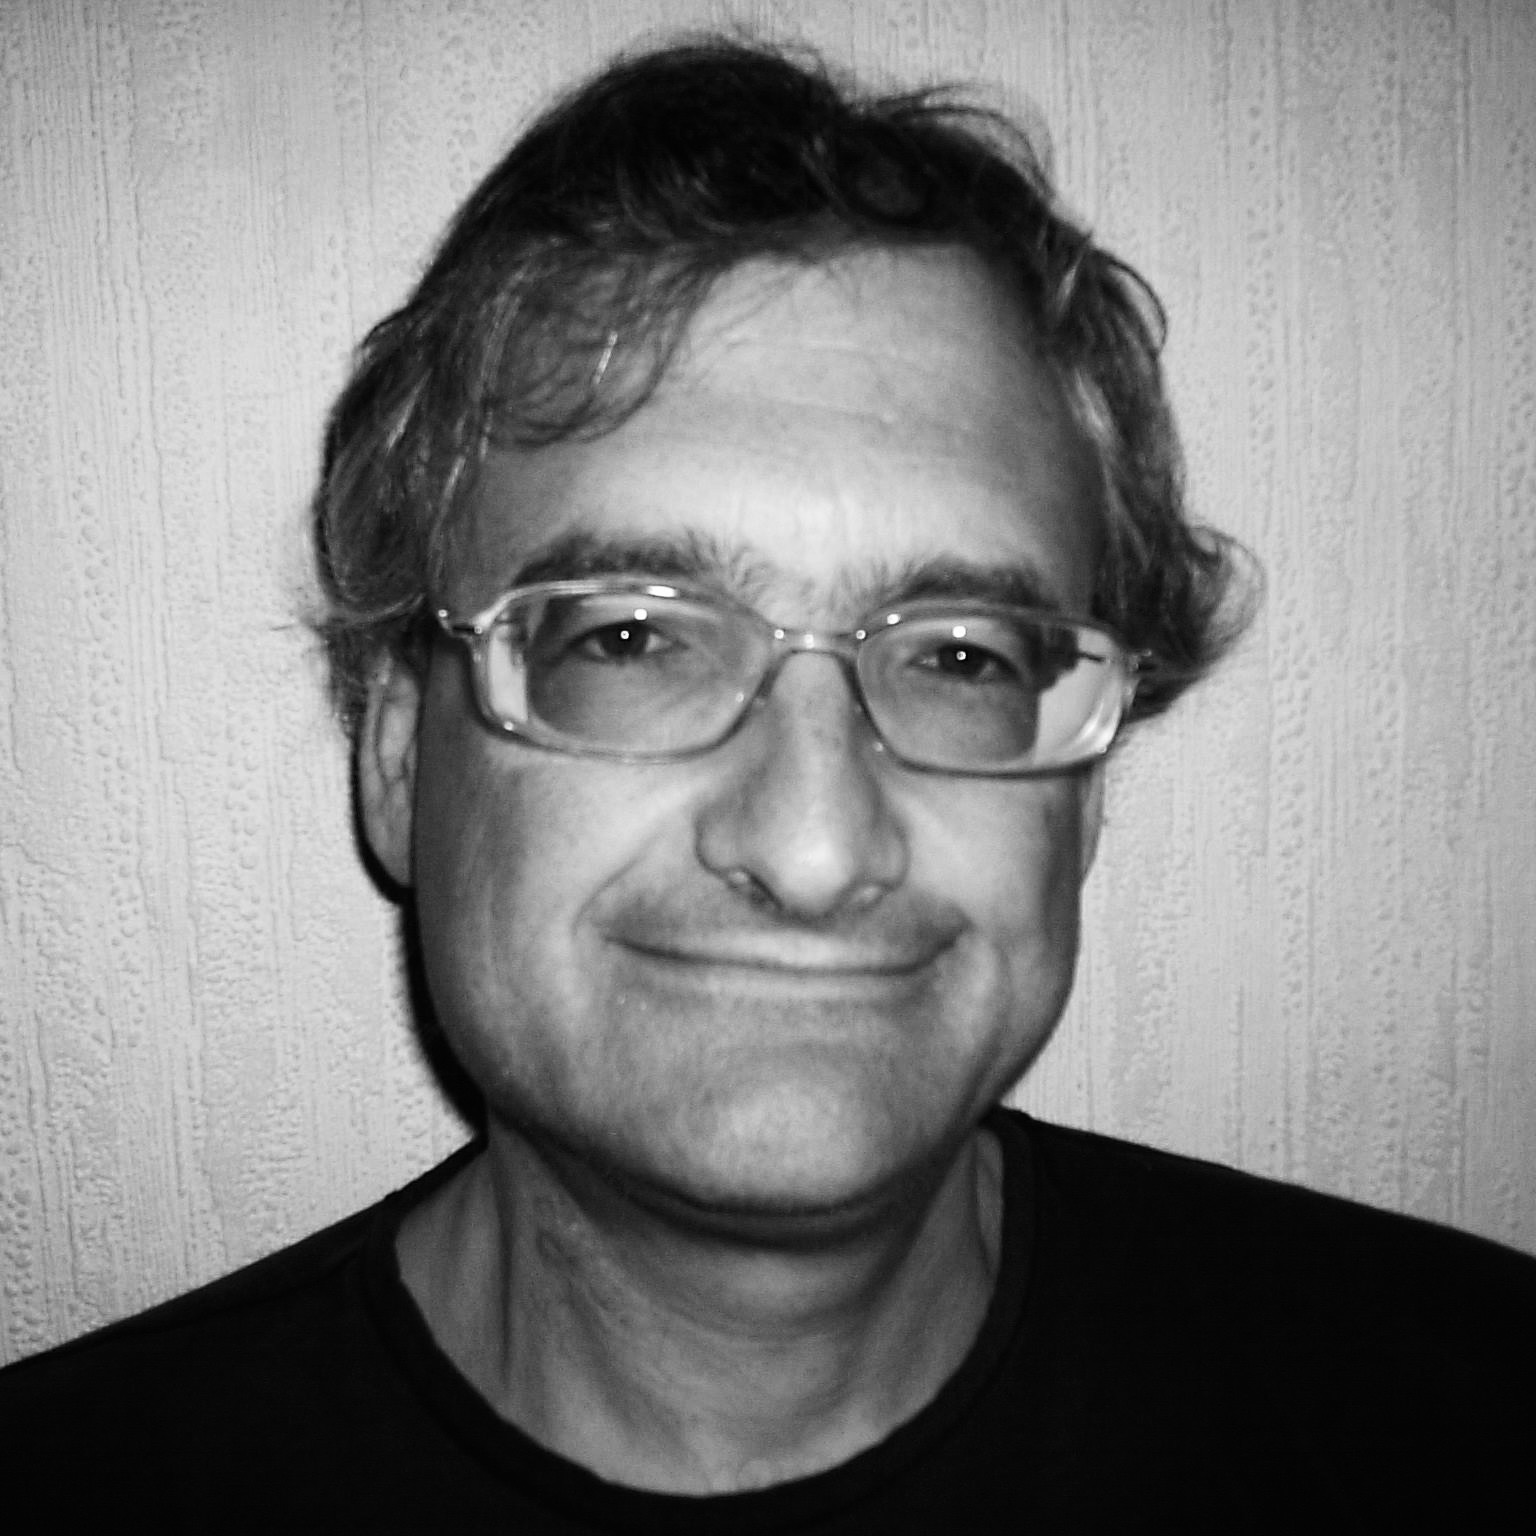
\includegraphics[height=100px]{content/day3/ehud-hs-bw.jpg}
\end{center}

\noindent
{\bfseries Abstract} 

Natural Language Generation (NLG) systems have different characteristics than
other NLP systems, which effects how they are evaluated. In particular, it can be 
difficult to meaningfully evaluate NLG texts by comparing them against gold-
standard reference texts, because (A) there are usually many possible texts which 
are acceptable to users and (B) some NLG systems produce texts which are better 
(as judged by human users) than human-written corpus texts. Partially because of 
these reasons, the NLG community places much more emphasis on human-based 
evaluations than most areas of NLP.

I will discuss the various ways in which NLG systems are evaluated, focusing on 
human-based evaluations. These typically either measure the success of generated 
texts at achieving a goal (eg, measuring how many people change their behaviour 
after reading behaviour-change texts produced by an NLG system); or ask human 
subjects to rate various aspects of generated texts (such as readability, accuracy, 
and appropriateness), often on Likert scales. I will use examples from evaluations I 
have carried out, and highlight some of the lessons I have learnt, including the 
importance of reporting negative results, the difference between laboratory and 
real-world evaluations, and the need to look at worse-case as well as average-case 
performance. I hope my talk will be interesting and relevant to anyone who is 
interested in the evaluation of NLP systems.

\vspace{3em}\par 

\vfill
\noindent

{\bfseries Biography} 

Ehud Reiter is a Professor of Computing Science at the University of Aberdeen
and also Chief Scientist of Arria NLG. He has worked on natural language generation 
for the past 30 years, on methodology (including evaluation) and resources as well 
as algorithms, and is one of the most cited authors in NLG. His 2000 book Building 
Natural Language Generation Systems is widely used as an NLG textbook. Dr Reiter 
currently spends most of his time trying to commercialise NLG at Arria (one of the 
largest specialist NLG companies), which grew out of a startup he cofounded in 
2009.
\newpage
